\documentclass[11pt,a4paper,onecolumn,oneside,notitlepage]{article}
\usepackage[utf8]{inputenc}
\usepackage[english]{babel}
\usepackage{amsmath}
\usepackage{amsfonts}
\usepackage{amssymb}
\usepackage{graphicx}
\usepackage{hyperref}
\usepackage{subcaption}
\usepackage[table,dvipsnames]{xcolor}
\usepackage{siunitx}

\usepackage[left=2cm,right=2cm,top=2cm,bottom=2cm]{geometry}

\usepackage[backend=biber, %% Hilfsprogramm "biber" (statt "biblatex" oder "bibtex")
style=authoryear, %% Zitierstil (siehe Dokumentation)
natbib=true, %% Bereitstellen von natbib-kompatiblen Zitierkommandos
hyperref=true, %% hyperref-Paket verwenden, um Links zu erstellen
]{biblatex}
\addbibresource{paper.bib}

\author{Oliver Tautz\\
	\begin{small}
		Deep Learning for Natural Language Processing -- SS21 -- Philipp Cimiano and Philipp Heinisch
	\end{small}
}
\title{Finetuning the T5 for Frame Identification}


\setlength\parindent{0pt}


\begin{document}
	\maketitle
	
	\section{Introduction}
Transfer learning with powerful, pretrained transformers is used to produce state-of-the-art results in many natural language processing tasks. \citep{wolf-etal-2020-transformers} For this assignement a relatively new transformer, the T5 \citep{T5} is used. The T5, which will be described in more detail in chapter \ref{method}, differs from encoder only, BERT-like \citep{bert} models as it uses an encoder-decoder architecture and can natively solve text-to-text problems. It was shown that many NLP tasks can be translated to such text-to-text problems and solved by a fine tuned version of the T5.\citep{T5}\\


The proposed shared task by \textit{webis} \citep{webis_task} is called frame identification. This is a classification task on full, natural text input. Each example text is an argument, which is labeled with its primary frame. The frame is a particular perspective of the argument which emphasizes an aspect of the associated topic. An example could be the frames ‘economics’, ‘job market’, or ‘education’ for an argument about a school reform. Frames are ambiguous and can be difficult to label even for humans. An automated system solving the task could be used by social scientists to gain more insight into what frames people respond to and evaluate what topics are important to the public or expose fraudulent abuse of framing in political debates.\\

As there is an almost unlimited number of frames a standard classification approach is limited to ones it has already seen and was provided enough data about. Thus the generative abilities of the T5 are explored for solving the task posed as a text-to-text problem, with mixed results, showing some promise but underperforming in comparison to already established techniques. 

		
\section{Related work}
The approach implemented by the task organizers \citep{webis_task_paper} uses an unsupervised clustering algorithm on heavily preprocessed input and achieves a macro weighted f1-score of \num{0.28}.\\

Another established approach to solve  NLP classification tasks is to use a pre-trained transformer to produce word embeddings from text and train a classifier on top of that , for example a KNN classifier. BERT was used\citep{bert_frame_ident} to great effect on the \citep{bert_dataset} dataset. Better results were achieved by also fine tuning BERTs embeddings, reaching \num{91.26} accuracy.  


\section{Method}
\label{method}

\subsection{Model}
The T5 is chosen because we can solve frame identification as a text-to-text task, which removes the general limitation of only being able to predict frames already considered while labeling. With great generalisation the model could theoretically be able to predict frames on general arguments on topics not in the training set. It is an encoder-decoder transformer using a standard architecture with stacked blocks of  self attention layers and fully-connected feed-forward networks in the encoder. For the decoder a normal attention layer is added. Regularization mechanisms, namely dropout and layer normalization are used in addition to resnet-like skip-connections.\citep{T5} Checkpoints trained on an unsupervised task on the large C4 \citep{2019t5} dataset are used as a starting point for training.\\

The \textit{keras} \citep{keras} T5 implementation and weights of \textit{huggingface transformers} \citep{wolf-etal-2020-transformers} are used.


\subsection{Problem Definition}

As the T5 can solve text-to-text tasks a very simple problem definition is chosen. Input \textbf{x} is the full argument as natural text, prediction target and label \textbf{y} is the text representation of the frame. A pair \textbf{(x,y)} is called an argument or sample subsequently. 
\subsection{Data}
\label{subsec:data}
The dataset used \citep{webis_task_paper}  comes with a lot of fields per sample, most of which are ignored. Used fields are ‘premise’, ‘conclusion’ and ‘frame’. Concatenating ‘premise’ and ‘conclusion’ forms input \textbf{x}. The frame field can be used without processing as label \textbf{y}. There are \num{12326} labeled arguments in the dataset. The frames are very unevenly distributed with some labels being present only once, and the most prominent frame 'economics' counting 119 samples.

\subsection{Preprocessing}
Experiments adding the task specific prefix 'summary' \citep{T5} to the input showed no effect. So minimal processing is used as described in  \ref{subsec:data}. The dataset is split before training into train-, test- and validation set with a split ratio of \num{0.2}, resulting in test-size of \num{2466} and val-size of \num{1973} respectively. The split is done in a stratified fashion, making a special case for samples with unique frames and distributing them according to the split ratio among train, test and val set. Arguments with rare frames, counting less than five samples are disregarded for training to achieve a more stable training signal, resulting in a train-set of \num{5351} samples. For training and predicting the input is tokenized by the T5Tokenizer \citep{wolf-etal-2020-transformers}, also padding and truncating sequences to the T5s max length of \num{512} tokens. 

\subsection{Training Setup and Hyperparameters}


\begin{figure}
     \centering
     \begin{subfigure}[b]{0.48\textwidth}
         \centering
         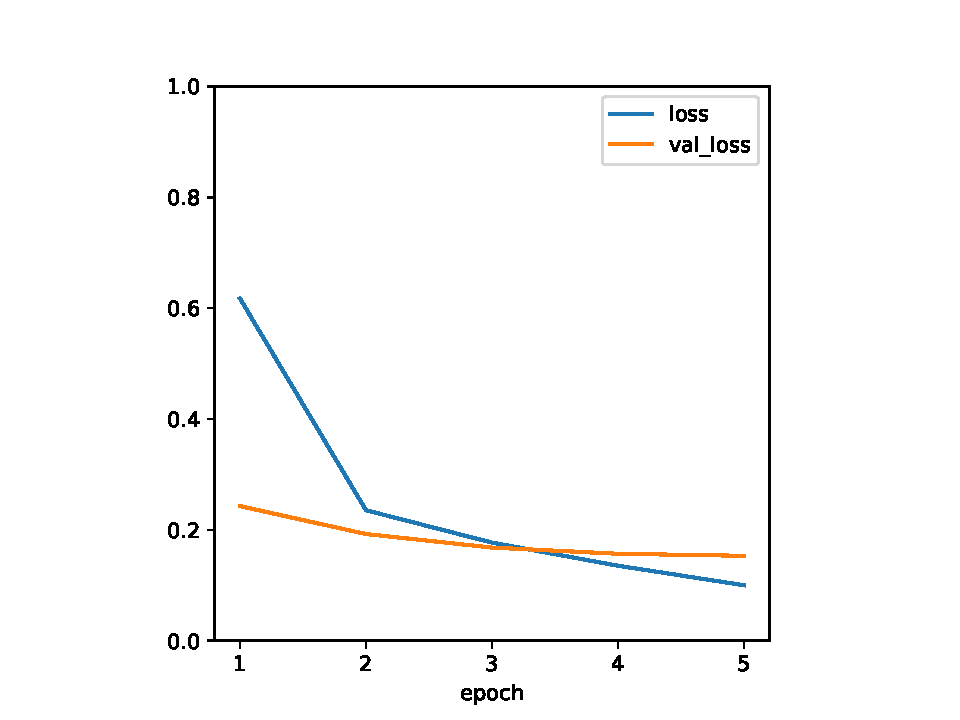
\includegraphics[width=\textwidth]{graphics/loss_base.pdf}
         \caption{t5-base}
         \label{fig:y equals x}
     \end{subfigure}
     \begin{subfigure}[b]{0.48\textwidth}
         \centering
         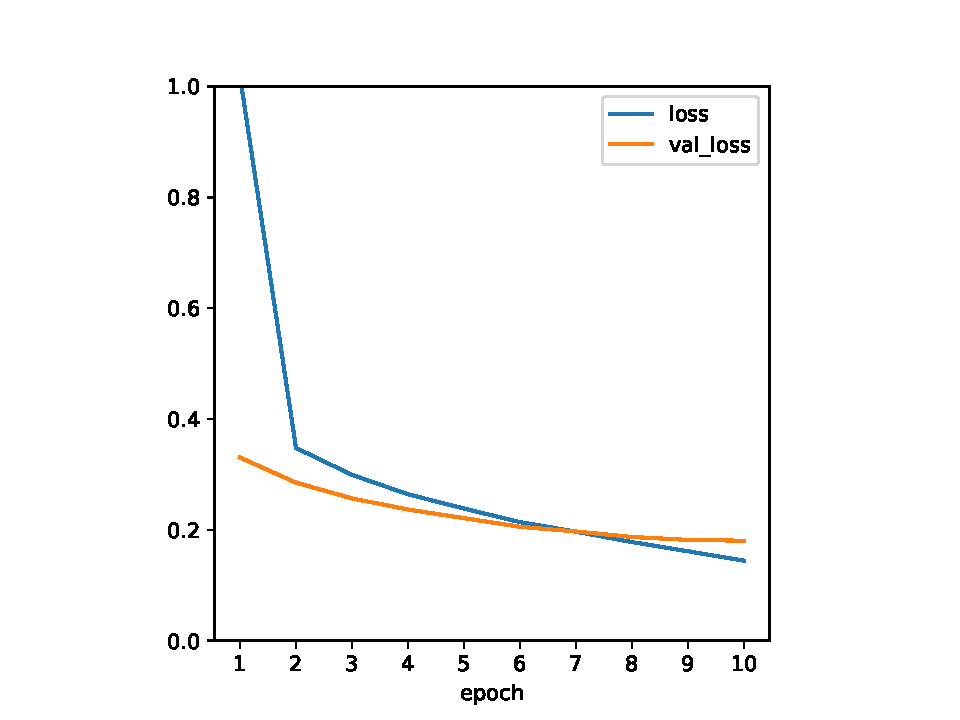
\includegraphics[width=\textwidth]{graphics/loss_small.pdf}
         \caption{t5-small}
         \label{fig:three sin x}
     \end{subfigure}
     \hfill
        \caption{learning curves of crossentropy loss}
        \label{fig:loss}
\end{figure}


Two models are trained, one starting from the provided, pre-trained checkpoint ‘t5-base’ and one starting from ‘t5-small’. The ‘t5-small’ is a smaller version of the T5. The base model is trained for \num{5} epochs, the small one for \num{10} epochs optimized by ADAM \citep{kingma2017adam} with a small, constant learning rate of \num{1e-4} and cross entropy loss. A batch size of 6 and 24 is used for the base and small model respectively. Both batch sizes are smaller than in the T5-paper but are chosen to be suitable for training on \textit{google colab}. Learning curves can be seen in figure \ref{fig:loss}. They show symptoms of overfitting after a few epochs for both models, quicker and more pronounced for the base model. Training is stopped early to improve validation and test performance.

\section{Evaluation}
\subsection{Metrics}
Three metrics are computed on the test set. To roughly compare to the BERT-classifier the ‘full lexical accuracy’, which means accuracy on all test samples, is computed. To compare to the task organizers clustering the macro-weighted f1-score is used. This is the mean of f1-scores per class, weighing them all equally regardless of size. For both the output is trimmed to text without padding and a prediction counts as correct only if the predicted and label string match. Because the T5 generates the frame text these are unsatisfying metrics as it can produce similar, yet not identical results. Therefore in addition the ROUGE-1 f1 \citep{rouge} score is computed. This metric is usually used to compare the similarity of full text summaries but is also applicable here. It is less harsh, as e.g. the prediction ‘popular opinion’ for a ‘public opinion’ labeled sample would be counted as partially correct. The T5 could still predict semantically similar frames, which is disregarded by both metrics.

\subsection{Results}


		\begin{table}
			\begin{center}
				\begin{tabular}{|l|c|c|c|}
					\hline
                    \textbf{Model} & \textbf{f1-macro}  & \textbf{Accuracy} & \textbf{Rouge1-f1}\\
					\hline
					\hline
					\hline
					t5-base 3 epochs & 0.111 & 0.295 & 0.322\\
                    \rowcolor{ForestGreen}
					t5-base 5 epochs & 0.192 & 0.429 & 0.449\\
					\hline
                    t5-small 5 epochs & 0.025 & 0.118 & 0.148\\
                    \hline
					t5-small 10 epochs & 0.127 & 0.316 & 0.338\\
					\hline
				\end{tabular}
			\end{center}
			
			\caption{results on test set}\label{tab1}
		\end{table}


Metrics computed on the test set can be seen in table \ref{tab1}. Although seemingly overfitting the training data, shown by diverging train- and validation-loss curves in figure \ref{fig:loss} the models continue to improve their test scores. The small model takes longer to reach a reasonable score. Accuracy, albeit evaluated on a totally different dataset, is low across the board compared to the BERT-classifier \citep{bert_frame_ident} , reaching  a maximum of 0.43 for the base model. ROUGE scores are only marginally higher, meaning most prediction hits are accurate and not diffuse ones.
The best model achieves an f1-score of 0.192 on the test set, also notably worse than the clustering approach of \citep{webis_task_paper}. The bigger model reaches significantly higher scores than the ‘t5-small’, both still unusably low. Training time was relatively short, with the base model needing 440s/epoch and the small one taking only 140s/epoch on a \textit{Tesla P100} with 16GB of VRAM.


\section{Conclusion}
The fine tuned T5 underperformed in comparison to both established classification models, but the results are still promising. In search of a general classification approach, predicting text instead of a class removes the limit of predefined classes and could leverage language understanding of machine learning models on another level. On this particular task there are lots of opportunities to explore. The rapid overfitting problem which is typical for high capacity model finetuning should be met with different techniques such as learning rate schedules, data augmentation, more balanced datasets and ‘gradual unfreezing’ which were out of scope for this assignment. \\

Without those techniques it was not possible to produce usable results. Generating the frame text seems to be a more difficult problem, requiring a better adapted model or training routine to be solved. The small model exhibited less overfitting problems but its reduced capacity did not seem fit to the task. The normal ‘t5-base’ improved quickly but could not generalize well enough, overfitting quickly. For subsequent research the full 't5-base' or even the here not explored 't5-large' model is recommended .



\printbibliography
\end{document}
